\documentclass{acm_proc_article-sp}
\usepackage{hyperref}

\begin{document}

\title{The Wikipedia Adventure: an Interactive Tutorial for New Wikipedia Users\titlenote{This is a class report for CS 294-78 ("Special topics on Technologies for Education and Learning at Large Scale") and SCMATHE 220c ("Science and Mathematics Education: Designing  Educational Technologies") at University of California, Berkeley created in Spring 2012.  All rights are waived under the Creative Commons Zero Waiver (CC0). This is not a peer-reviewed work.}}

\numberofauthors{1}
\author{
\alignauthor
Derrick Coetzee \\
       \affaddr{University of California, Berkeley}\\
       \affaddr{Berkeley, California, USA}\\
       \email{dcoetzee@eecs.berkeley.edu}
}

\maketitle

\begin{abstract}
New contributors to Wikipedia face daunting technical and social challenges, contributing to ongoing decline in editor retention and systemic bias in article content. The Wikipedia Adventure is a web-based interactive tutorial for new users that leads them through learning essential basics in a safe game-like environment, and can extend to instruction on advanced skills. All interactions are tracked and linked to the user's real Wikipedia account, where their performance can be evaluated based on contribution logs. We constructed a prototype that demonstrates the feasibility of all essential features with a subset of lessons, and gathered preliminary usage data and feedback from testers gathered from an expert user pool.
\end{abstract}

% A category with the (minimum) three required fields
% \category{H.4}{Information Systems Applications}{Miscellaneous}
%A category including the fourth, optional field follows...
% \category{D.2.8}{Software Engineering}{Metrics}[complexity measures, performance measures]
% \terms{Theory}
% \keywords{ACM proceedings, \LaTeX, text tagging} % NOT required for Proceedings

\section{Motivation}

Since 2007, Wikipedia has experienced declining editor participation and retention, as shown in Figure~\ref{fig:retention}. Suh\cite{Suh:2009} cites ``exclusion of newcomers and resistance to new edits'' as possible explanations. Personal experience shows new editors often either can't figure out how to edit Wikipedia, or have negative experiences due to their unfamiliarity with the site and its policies, and stop editing. Learning policy thoroughly is an overwhelming prospect---just the key policies and guidelines fill a 270-page book---and there is little guidance regarding which policy is most important to learn first. The goal of this project is to help new Wikipedia users to generate quality content by using an interactive, web-based tutorial to teach basic Wikipedia editing and policies.

\begin{figure}
\centering
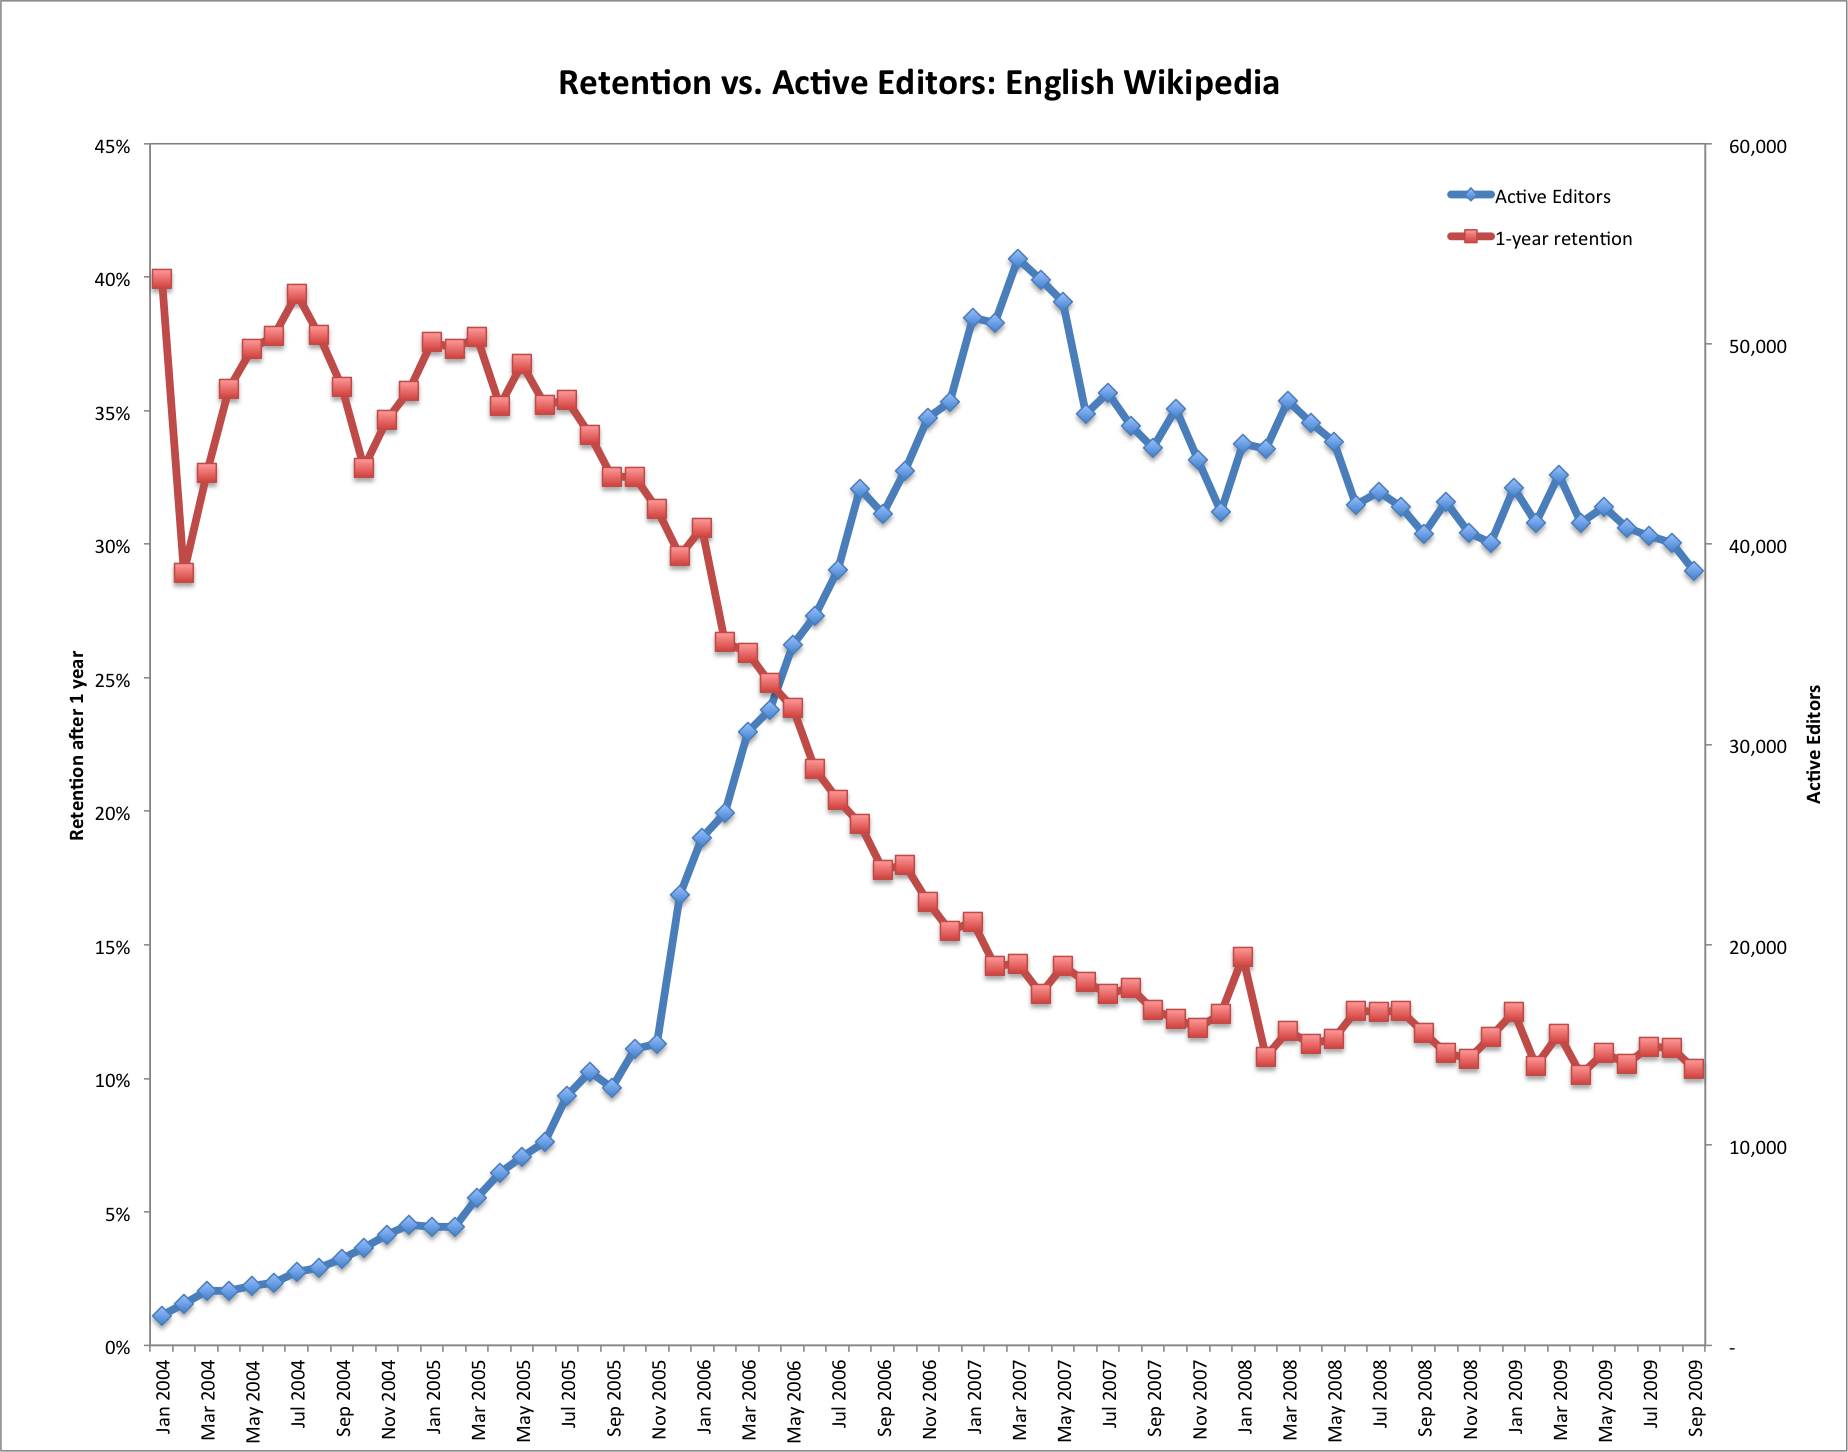
\psfig{file=images/Enwp_retention_vs_active_editors.png, width=\columnwidth,}
\caption{Active editors and editor retention, 2004-2009. Active editors peaked in early 2007 and the one-year editor retention rate has fallen to 10\%. Source: Wikimedia Foundation Editor Trends Study.  
\url{http://strategy.wikimedia.org/wiki/File:Enwp_retention_vs_active_editors.png}}
\label{fig:retention}
\end{figure}

\begin{figure*}
\centering
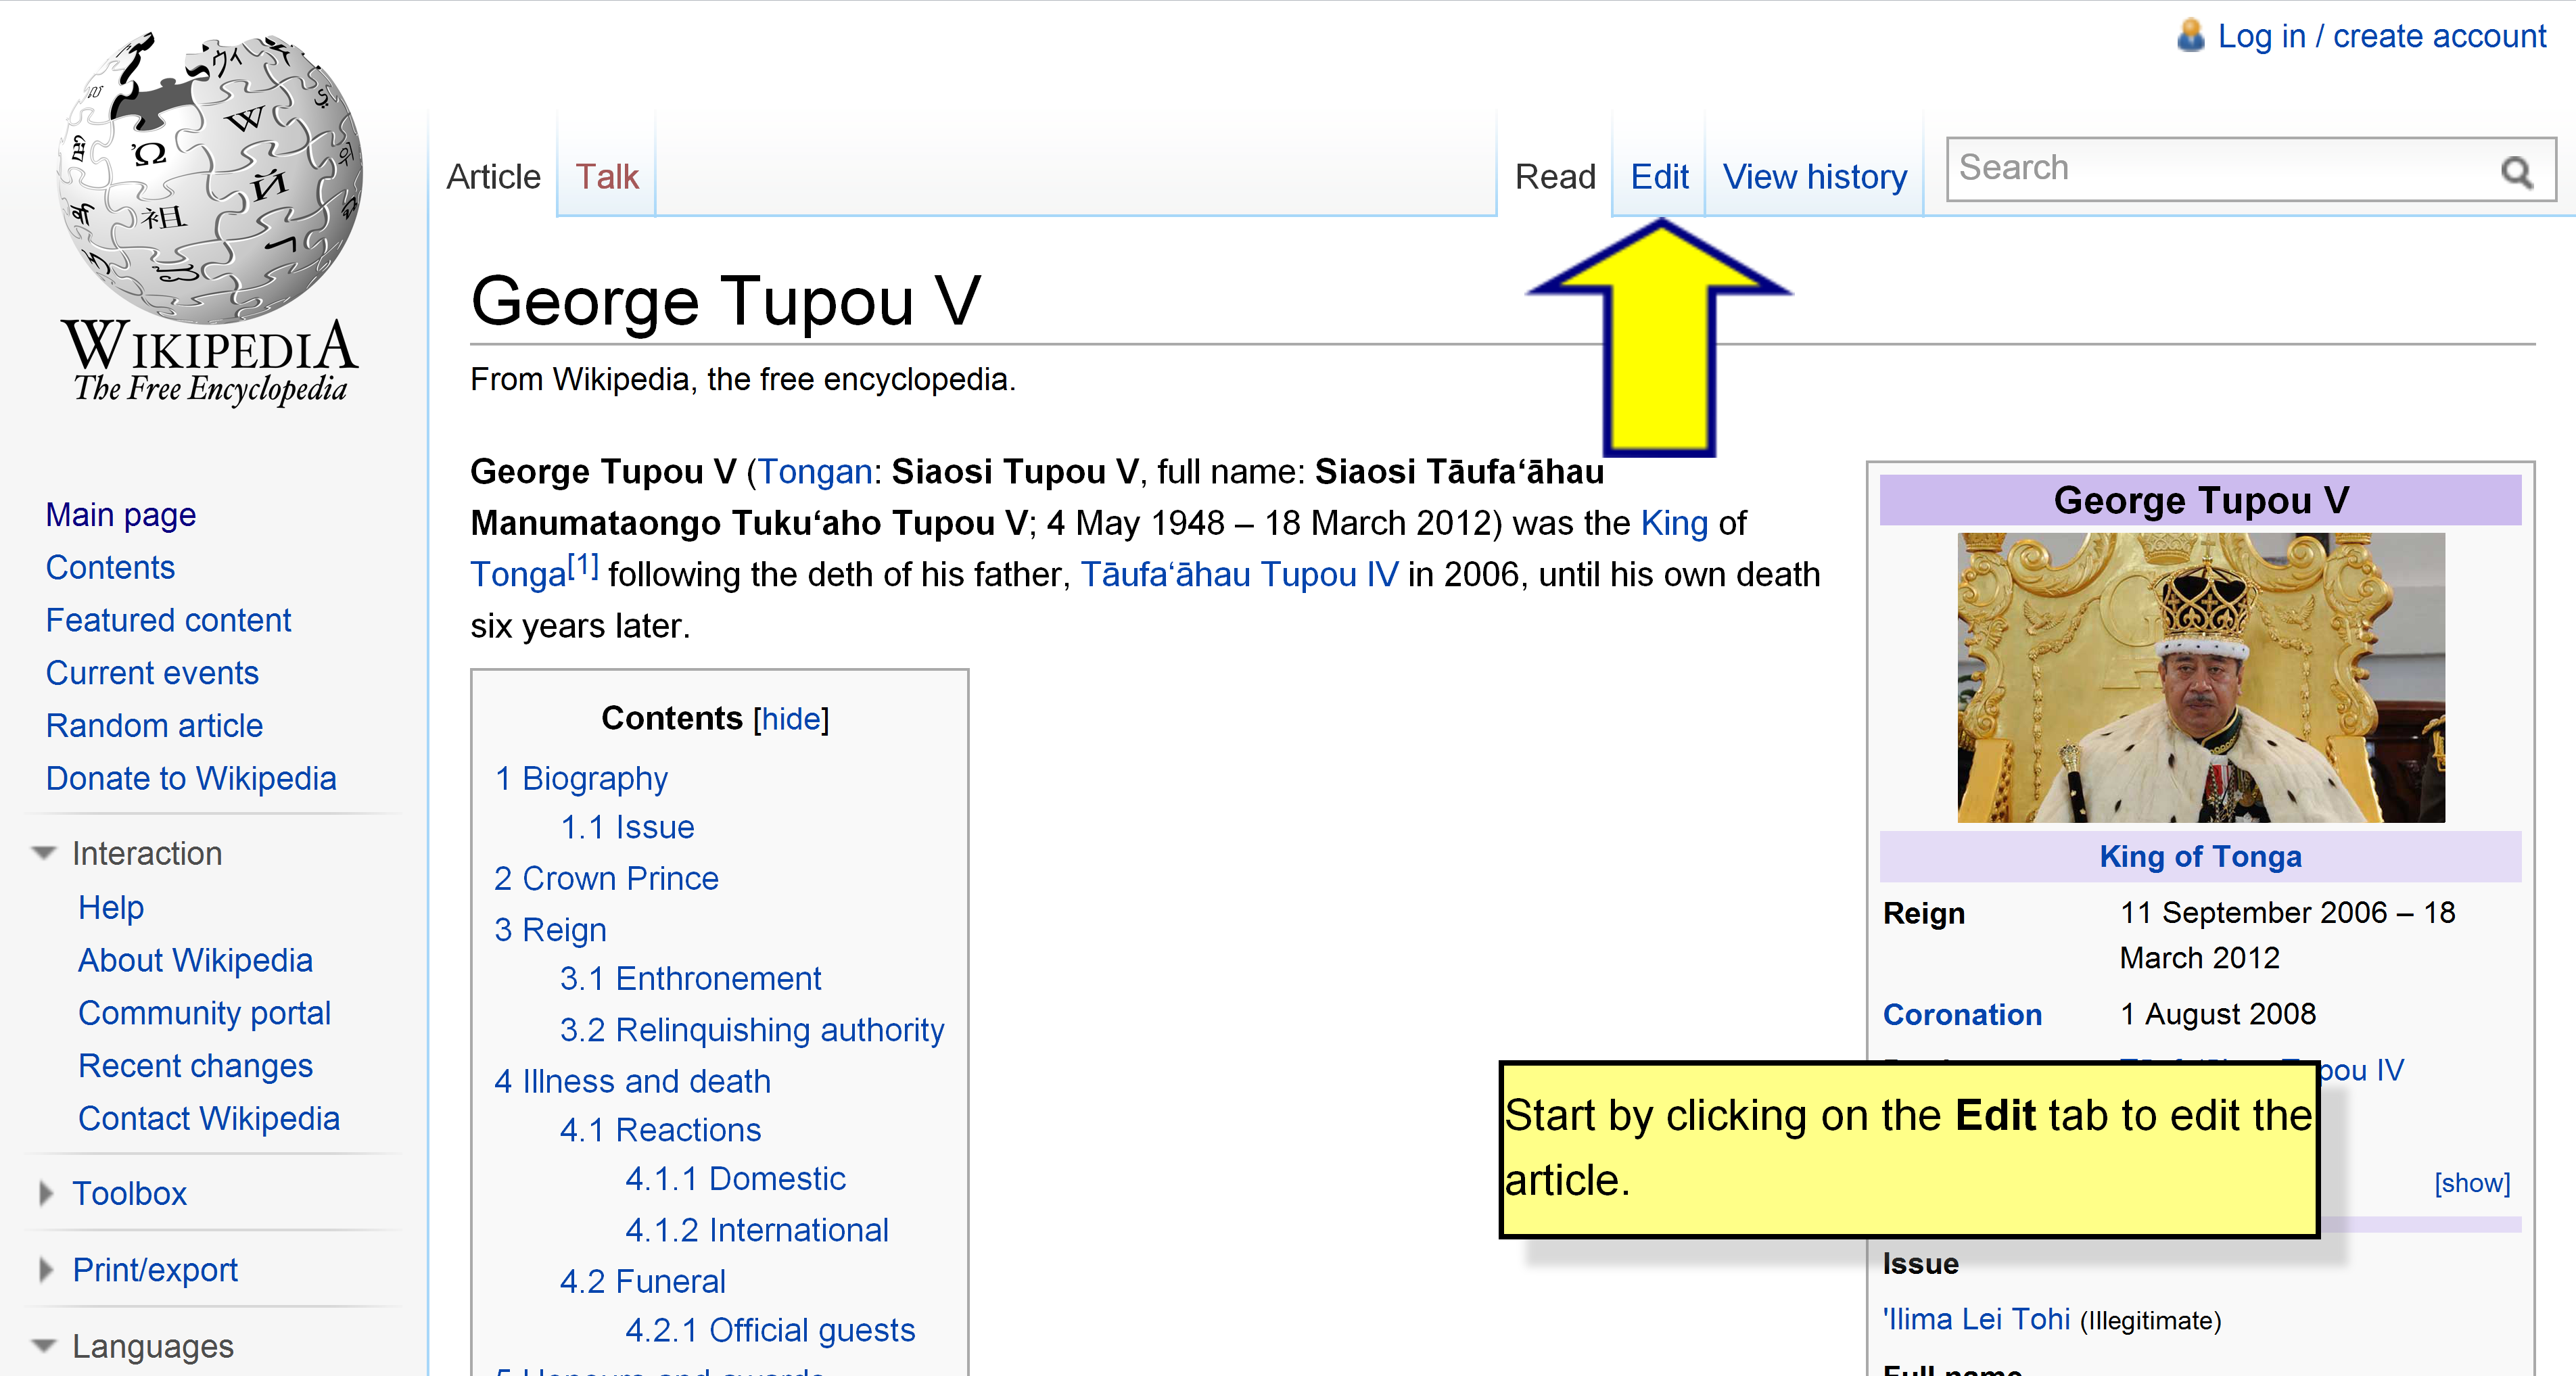
\psfig{file=images/wikipedia_adventure_big.png, width= 2 \columnwidth,}
\caption{Screenshot from first level of The Wikipedia Adventure. The interface is identical in appearance to the real Wikipedia interface, except that instructions are overlaid instructing the user to click on the edit button. }
\label{fig:screenshot}
\end{figure*}

From a user perspective, the motivation to contribute to Wikipedia can come from many sources. Some are financially motivated, seeking to generate publicity for their business, band, or professional works, or to increase web traffic to their website via links. Some are egotistically motivated. Some are students participating as a course requirement. Some are motivated by a desire to ensure articles are accurate, or to spread awareness of a topic or point of view. Some are motivated by a desire to make an impact, some by a desire to attain status in the Wikipedia community, and some by a desire to spread knowledge to others. Motivations of Wikipedia editors have been explored by numerous researchers; a good source is Kuznetsov,\cite{Kuznetsov:2006} which qualitatively explored a number of intrinsic and extrinsic motivating factors such as altruism, reciprocity, community, reputation, and autonomy.

Likewise, the demographics of new Wikipedia users are diverse, coming from all age groups and all regions of the world. Thirteen-year olds in the US routinely contribute to articles on popular culture, and retiree professors abroad who are speakers of English as a second language contribute as experts in their fields. Some carry PhDs in computer science, while others are barely capable of using a web browser. Glott\cite{Glott:2010} gives a survey of Wikipedia user demographics.

Teaching effective Wikipedia editing to such a diverse audience is a challenge: major differences in educational backgrounds and technical skill mean that tasks which are remedial for one audience (such as account creation) are challenging for others. This means the tutorial must be flexible enough to allow users to learn about basic tasks without boring more adept users. The primary strategy used to address this is allowing skipping of early lessons based on answers to questions (for example, users who already have an account are not instructed how to create one).

Another challenge is that many of the motivations listed above are short-term, in the sense that they just want to write a single article (e.g. on their company) or fix a single problematic article and are not interested in investing time and effort in the lessons needed to become a good long-term contributor. Unlike in a classroom environment, users cannot be compelled to complete the tutorial. An effective tutorial must recognize this by teaching the bare essentials needed for a contributor to begin achieving their immediate goal before they lose interest, but also encourage them to return when they encounter new barriers. One way to encourage return is to give a preview of what is taught by future lessons before they depart; another is to place links to lessons on Wikipedia, in the context where they are most useful.

\section{Existing educational resources}

One way for new users to learn to use Wikipedia is to simply start using Wikipedia; this is explicitly encouraged by Wikipedia's ``be bold'' guideline. Upon encountering difficulties, they receive feedback from other users (see Figure~\ref{fig:talktemplate}), consult help pages, ask for help, and experiment. If their understanding is incomplete, they receive further feedback when attempting the task again. Because learning is motivated by successful completion of the task immediately at hand, this facilitates in-context learning that is targeted and personally relevant in the sense of Olfman.\cite{Olfman:1991}

\begin{figure}
\centering
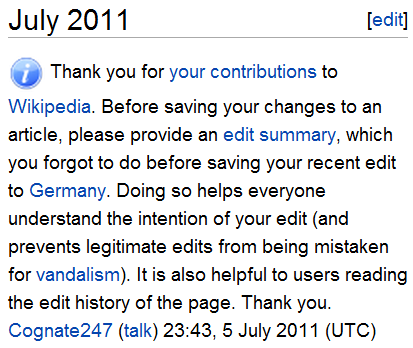
\psfig{file=images/talk_page_message.png, width=2.5 in,}
\caption{A standardized talk page message reminding a user to enter edit summaries when editing. Feedback from other users provides targeted in-context learning, but is costly.}
\label{fig:talktemplate}
\end{figure}

These mechanisms can be highly effective for experienced users who know which of these resources to exploit and at what times, but for new users, these resources are either difficult to locate, difficult to use, or too many options are offered, leading to confusion. Moreover, the written help pages are not interactive, forcing users to experiment on the live site in order to "test out" what they have learned. Some users cause damage, while others, fearing they will break something, are reluctant to experiment, especially in complex articles using sophisticated markup.

Personalized feedback is slow and costly. All new users repeatedly encounter the same issues. Experienced users have resorted to using impersonal standardized messages (\emph{templates}) to provide feedback, as shown in Figure~\ref{fig:talktemplate}. In an interactive tutorial, feedback can be given instantly, and no manual effort is required.

Help and policy pages on Wikipedia, like articles, are structured as a web: each one links to many other help and policy pages. While valuable for exploratory learning for long-term users, new users who just want to learn enough to complete their short-term task are frustrated by this, not knowing which of the many linked documents will help them complete the task at hand correctly.

Another limitation of the standard interface is that the main encyclopedia is already well-developed. Notari,\cite{Notari:2006} on motivating students to participate in class wikis, emphasizes the need for a ``launch activity'' which is ``motivating, easy , and quickly achievable.'' Most substantive article-writing activities no longer fall under this description, necessitating the invention of artificial tasks. Although not as motivating as real activities, artificial tasks in a fake environment can be repeated by each user uniformly without consequences, and may be simpler than corresponding tasks on the real project.

\section{Design and learning goals}

The proposed tutorial would simulate the experience of the real Wikipedia website, but not affect the real site, and so is ``insulated from real consequences.'' \cite{Garris:2002} Instead of a complex web of pages, users will be given scripted instructions and a limited number of options at each point, with a mostly linear flow (links/options that are permitted are highlighted, while other links/options are nonfunctional).

The goal of the introductory lessons is to help the user learn enough to complete their desired short-term task successfully, while also teaching them enough to seek additional help as needed, either through additional lessons or through existing channels on Wikipedia. As emphasized by Olfman,\cite{Olfman:1994} it's important for initial training to include a combination of procedural training (technical how-to information) and conceptual training (helping new users to build a mental model of the site). In particular, basic concepts like how articles are communally edited and their content determined by consensus are essential for all users to understand.

After completing the initial lessons, which introduce basic editing and help tools and share a linear narrative, the user has the option of choosing from a pool of largely independent advanced lessons (exploring phase). These lessons serve two purposes: they allow users interested in exploratory learning and becoming long-term users to continue learning about subjects that interest them, and they allow users who have trouble in a particular area to learn more about that area. In both cases, they help developing editors to become expert, long-term users. By allowing direct web links to lessons, other users can suggest particular lessons, and help pages can link to related lessons. For particularly complex topics, prerequisites can be implemented where one lesson is recommended or required to be completed before another.

The practice of having an initial, easy linear stage followed by a ``wide open'' exploratory space of more difficult stages, illustrated in Figure~\ref{fig:airship}, is common in games, such as in the Final Fantasy series, where players are initially ``railroaded'' along a linear set of locations while learning the mechanics of the game, but are eventually given access to an airship that allows any location in the world to be easily visited in any order (although there may still be prerequisites---quests which must be completed before other quests can be started). For this reason we refer to this as an \emph{airship structure.} Acquiring the airship can be motivating in itself because of the new freedom it offers; in the same way, the tutorial can create motivation to complete introductory lessons by informing the user that once they ``graduate,'' the pool of advanced lessons will be unlocked.

\begin{figure}
\centering
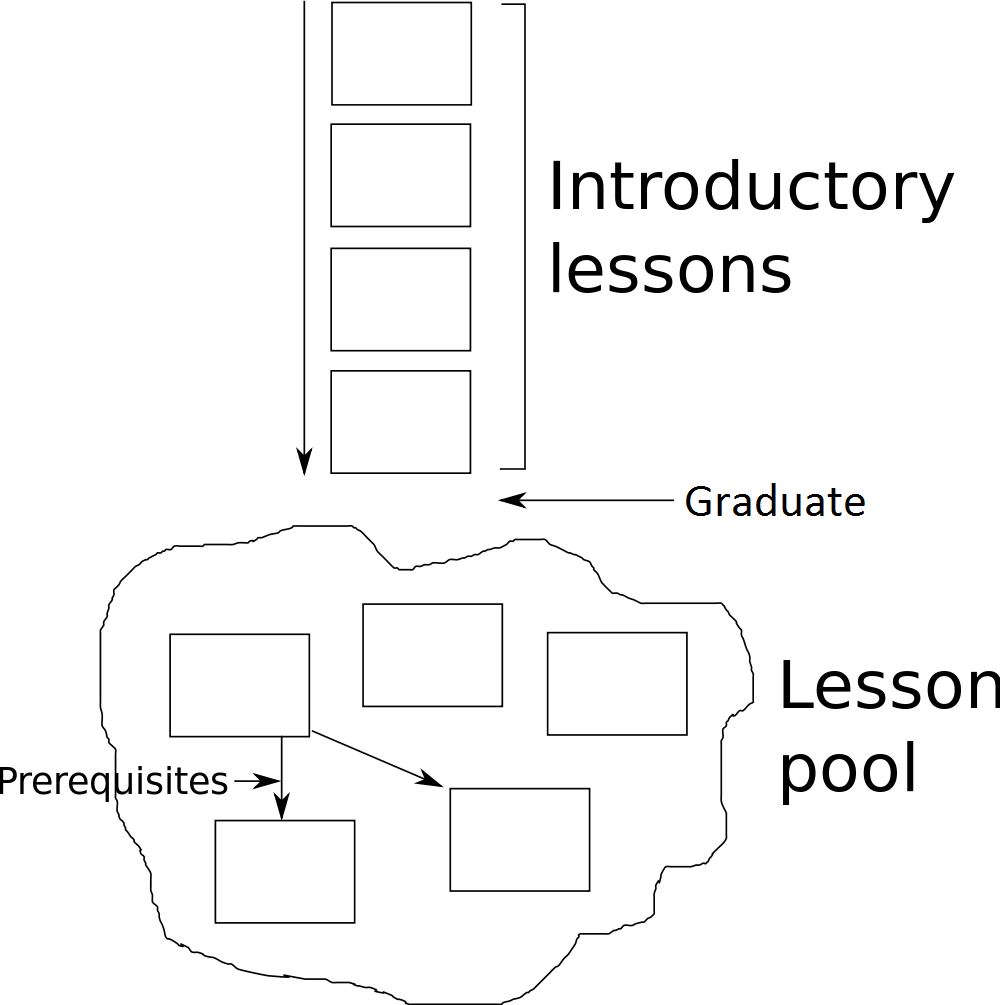
\psfig{file=images/airship.png, width=\columnwidth,}
\caption{Airship structure. Introductory lessons teach essential concepts, then the user ``graduates'' to the advanced lesson pool, which is much larger and can be explored freely to learn concepts needed for the task at hand, subject to prerequisite constraints.}
\label{fig:airship}
\end{figure}

At certain stages, the user will need to enter text, which needs to be evaluated for compliance to policies, such as "neutral point of view." Because it's not technically feasible to perform this evaluation on arbitrary text, the user would instead be presented a small number of text options, and the option they select is entered for them. Figure~\ref{fig:multiplechoice} shows a user selecting a username in compliance with username policy. If their selection is incorrect, they are immediately informed of the reason why and asked to choose again.

\begin{figure}
\centering
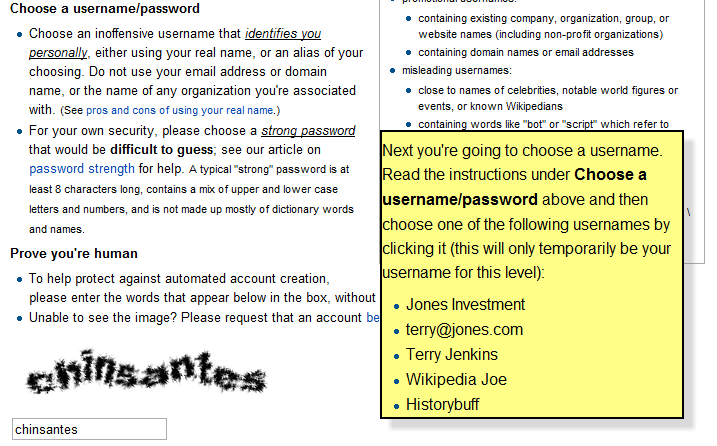
\psfig{file=images/multiple_choice.png, width=\columnwidth,}
\caption{A user is given several usernames and asked to choose one in compliance with username policy. If they select incorrectly, the option will be highlighted in red and an explanation will be given instantly.}
\label{fig:talktemplate}
\end{figure}

Other Wikipedia users have expressed an interest in translating the tutorial into other languages. This is no small matter, because each language has a separate Wikipedia project with its own community and rules, and different priorities regarding what is essential; effectively a complete lesson builder like the one described in section~\ref{sec:lessonbuilder} is needed to support this.

Negative feedback is controversial. On the real Wikipedia, users receive negative feedback for violating rules, eventually being blocked from editing entirely. The tutorial needs to illustrate that negative actions have negative consequences, without inadvertently encouraging negative actions. There are a couple ways to accomplish this: one is to show others receiving negative feedback in response to negative actions, and another is to give rapid feedback, immediately pointing out the negative action and ask the user to try again.

The introductory lessons are of special note because although all new users have a need for certain basic skills, differences in motivation and background may justify altering the approach. Tech-savvy users should be able to skip easy lessons, or else they will be bored and lose interest.  Financially motivated users may need instruction on the conflict of interest policy, whereas altruistic users require none. Lessons can be made more personally relevant, again in the sense of Olfman\cite{Olfman:1991} by using example content in the area of interest of the new user.

\section{Collaboration}

The tutorial described so far merely simulates communication between users, and is not effective at teaching real collaboration. Notari,\cite{Notari:2006} describing use of wikis in constructivist classrooms, places a heavy emphasis on collaboration, from the beginning developing a ``communication and comment culture'' with simple activities like commenting on one another's personal introductions.

One way to address this is to exploit the existing collaborative platform by directing students to complete tasks on the real Wikipedia such as creating a real user page or giving feedback on an article talk page, creating a hybrid tutorial experience. All lessons created so far have a ``Real Wikipedia task'' at the end meant to reinforce the learned concepts. However, this type of task must be tailored to avoid risk of damage to the real project or its users, limiting its utility.

Another method, not yet used, is to feature interaction among players---for example, one player could leave a talk page message in the tutorial and another responds to it. This generation of tutorial content by players can create more diverse content, at the risk of incorporating unsuitable or low-quality content.

\section{Drawing users in with game mechanics}

One important goal is to draw users in to the lessons, encouraging them to complete more of them rather than abandon the interaction. A variety of familiar game mechanics can be leveraged for this. Lessons can contain links to related lessons at the end of lessons, encouraging exploratory learning, and players can receive awards for completing lessons (based on number or perhaps for completing a group of related lessons). By displaying awards on the user's real Wikipedia user page, they are motivated by community reputation. A "high scores" chart comparing their performance to that of other community members may also be motivating. Mandatory prerequisite structures can act as an incentive: a player who wants to complete a particular lesson (perhaps because a special award is attached to it) will go through the necessary prerequisite lessons first, a process known in games as ``unlocking.''

Another interesting mechanic would be for players to complete certain tasks on the real Wikipedia, and receive ``credit'' inside the game for it, raising their score or unlocking additional lessons. This would act as a gentle push for users reluctant to make the jump from a safe environment to one with real consequences.

Another important goal is to encourage players to redo lessons that they may not have fully understood the first time. Drawing on games, one way to do this is with a score system that yields the most points for making good editing decisions. To make achieving the best score more challenging, available responses can be chosen randomly each time.

Paras\cite{Paras:2005} emphasizes the importance of incorporating periods of reflection into gameplay, since players do not normally reflect while in a state of flow. In games like Starcraft, this is accomplished by rich visualizations and replays of what occurred during the game that can be reviewed between games. Likewise, if our tutorial possesses a score system, it should allow a player to revisit their responses and where they gained and lost points between lessons, allowing them to identify areas for improvement. This will also create what Garris\cite{Garris:2002} refers to as a ``judgment-behavior-feedback loops,'' an essential advantage of games over passive instruction.

\section{Implementation}

In order to be broadly accessible to the diverse user base of Wikipedia, who already has web access, a web-based tutorial is intuitively advantageous. Running portably across major platforms and on hardware with poor performance is essential. Although some users only access Wikipedia from mobile devices, the editing interface on mobile devices is not usable at the present time, and so a mobile tutorial is unnecessary.

The interface of the tutorial needs to simulate the already-complex interface of Wikipedia itself, and remain up-to-date as that interface is modified. Major changes to the editing interface, for example,  are planned in the next year. The approach chosen to mitigate this was to base the tutorial on MediaWiki, the open source software used by Wikipedia, with other elements added on top using Javascript. By duplicating the content, settings, and extensions of the real Wikipedia, the interface can be made to precisely resemble that of the real website. 

Although it is intuitively appealing to integrate the tutorial directly into the main Wikipedia site, making it easily accessible and allowing more interaction between it and the real site, this also risks compromising the impression of safety offered by a clear simulation (and may in fact lead to damage to the actual project, in the event of errors). Moreover, changes in the underlying site would require continual updates to the script. Instead the tutorial was located at a separate domain, providing stability and safety.

In order to validate ownership of Wikipedia accounts, we use a reserved Wikipedia account and the MediaWiki API to send e-mail to their Wikipedia user containing a confirmation code, which is then entered into the tutorial. The confirmation code is a hash of their username together with a secret key. This ensures accurate association of accounts.

Users are encouraged to use a different password from their regular Wikipedia password. Passwords are protected using standard salting and key stretching techniques.

\section{User testing and assessment}

As with any software tool, the most valuable feedback comes from real users. The system is instrumented to track each action by users, allowing their progress to be assessed. User e-mails are requested, allowing follow-up surveys or interviews for qualitative feedback. Users create accounts which are tied to their Wikipedia accounts via a secure validation process, allowing their performance in the lessons to be correlated with their later contribution history as editors. Testing is expected to be an indefinitely ongoing process alongside real use.

New users can be recruited from a variety of existing venues that already deal with new users and answer their questions, including online chat, the Articles for Creation process, welcome messages, and the help desk page. Links can be added to the tutorial where suitable, and volunteers who deal with new users can be trained to link to relevant tutorial lessons.

Proficiency is assessed from a user's Wikipedia contribution by an expert Wikipedia user using a rubric, shown in Figure~\ref{fig:rubric}. The rubric highlights essential skills that are taught in the tutorial and can be observed. To deal with the fact some parts of the rubric don't apply to users who don't edit much at all, we define three \emph{participation categories}:

\begin{itemize}
\item Low participation (0): User made no edits to Wikipedia article content, or made only minor edits such as spelling corrections.
\item Medium participation (1): User made some major content contributions to Wikipedia, but had little to no interaction with other editors.
\item High participation (2): User made major content contributions to Wikipedia and interacted substantially with other editors.
\end{itemize}

The rubric indicates which items apply to which participation category, and scores can only be compared within a category. These scores can then be analyzed, for example by determining whether tutorial users have significantly higher scores, or by correlating them to a user's level of progress through the tutorial. This is not a controlled study because participants in the tutorial are self-selected, but it can offer a broad estimate of improvement while also pointing our issues in certain lessons.

\begin{figure}
\centering

\begin{itemize}
\item Correct use of syntax and formatting (medium and high)
    \begin{itemize}
    \item 0: User uses no markup/formatting or only uses it incorrectly.
    \item 1: User uses only the most basic formatting, or makes many mistakes while using formatting.
    \item 2: User is competent with basic to intermediate syntax and formatting, but might make a few errors.
    \item 3: User uses advanced syntax or formatting with few errors.
    \end{itemize}
\item Neutral point of view (medium and high)
    \begin{itemize}
    \item 0: User's writing is consistently blatantly biased, showing only one side of a topic and using strongly biased language.
    \item 1: User's writing mixes biased content with neutral content, or describes neutral facts using heavily biased language.
    \item 2: User's writing contains some bias or omissions, but overall presents an acceptably neutral account of the topic.
    \item 3: User's writing contains very little bias and effectively describes and integrates multiple points of view.
    \end{itemize}
\item Copyright policy (medium and high)
    \begin{itemize}
    \item 0: User only contributed content that violated copyright.
    \item 1: User's contributions included major blatant copyright violations, but also contributed original content successfully.
    \item 2: Some of the user's contributions were too closely paraphrased or some quotes were too long, but there were no major, blatant copyright violations.
    \item 3: All of the user's contributions were original or within the bounds of fair use.
    \end{itemize}
\end{itemize}

\caption{A portion of the rubric for assessing a user's proficiency based on their contribution history. Items are based on important policies and editing mechanics. Each item is labelled with the participation categories to which it applies (see text). The scores for each item are added to obtain an overall performance score.}
\label{fig:rubric}
\end{figure}

Only users in the same participation category can be directly compared. The number of users in each participation category can be used to assess overall participation level of the group.

\subsection{Preliminary usage and issues}

Because lessons are incomplete, new users have not yet been asked to
experiment with the system. Experienced Wikipedia users performed 
ad hoc testing and usage data and design suggestions were gathered.

A number of qualitative issues were observed in usage data. Users
sometimes became stuck---for example, when editing in the first lesson,
if it said they made the edit incorrectly, they couldn't see where in the text
they made an error. Highlighting errors more clearly and/or providing
hints to users who are stuck could be helpful. Users spent more time
on steps involving visual searching, and less on steps where the item
to click on was clearly indicated. A number of users
abandoned the interaction in the middle for unclear reasons, suggesting that a ``back'' or
``main menu'' button could give them a way out, in the event of frustration.

Several users suggested indicating when the
highlighted element is not present in the current window, for example by
adding ``scroll down'' and ``scroll up'' indicators. 

\section{Lesson builder}
\label{sec:lessonbuilder}

A vital component going forward will be to enable users who are not technically savvy to contribute new lessons to the lesson pool. This will dramatically increase breadth and depth of content, motivate recruiting, and allow content creators to learn by teaching. However, this also risks creating the same excess of options presented by the original website, particularly if multiple lessons cover the same topic. One way to address this is to leverage ratings by players to choose their favorite lessons, and display highly-rated lessons in each category at the top.

Users building lessons need to be able to identify elements of the page robustly without understanding the underlying markup. Ideally, the lesson builder would simply click on an element and a robust query identifying the element at that position would be derived automatically. Lessons follow a state machine, and lesson builders need to be able to identify lesson steps and transitions between steps based on user input. A visualization of this state machine may be effective. Lesson builders also need to be able to dynamically modify the page to create the appearance of the user's actions having an effect when in fact (for repeatability) this is not permitted. A history feature would be valuable to permit collaboration on lesson designs over time.

The lesson builder can be extended into a more complete toolkit allowing third parties to develop interactive tutorials for any website, or even for desktop applications. Appropriate abstractions would need to be created to remove the current implementation's strong dependency on Javascript.

\section{Status and future work}

Currently only a prototype with a subset of lessons is implemented. Although the prototype successfully
verifies the feasibility of the implementation mechanisms required, more content
must be generated to complete the introductory lessons and fully prepare new
editors for contributing. Advanced lessons can be added as they become available.

Ad hoc testing by experienced users has been performed, and usage data has been
gathered, which gives basic information like minimum lesson completion time,
but is not representative of the target user class. Proficiency assessment of
users in the control group is proceeding in parallel with development. More lessons must
be completed before proficiency assessment can meaningfully proceed for tutorial users.
Analysis will follow.

Motivating game mechanics such as a score system and user page awards are currently
unimplemented.

Currently lesson information is hardcoded in Javascript, which suffices for introductory
lessons, but advanced lessons need to address hundreds of detailed policies and
technical features. The lesson builder is essential to scale the project by distributing
the effort of building  a pool of advanced lessons among volunteers. The lesson
builder also provides a path to a tool that is useful in a more general setting.

\section{Conclusions}

We created a prototype that effectively demonstrates the technical feasibility
of building an interactive tutorial for new Wikipedia users, tracking usage and progress,
and linking users to their real Wikipedia accounts. Upon completion
of the lesson content, educational assessment can begin. The system serves both
to address a clear need of the Wikipedia project, and as a first application of a
more general system that can provide interactive education for a variety of
technological tools.

\section{Acknowledgments}
The Wikipedia Adventure is based originally on an idea and
initial design defined by User:Ocassi. Mock-ups
were done by User:Sonia. Several
other Wikipedia users and the staff of
CS 294-78 and SCMATHE 220c gave feedback following
review of the design and ad hoc testing.

\bibliographystyle{abbrv}
\bibliography{sigproc}  % sigproc.bib is the name of the Bibliography in this case

\end{document}
